
\section{Global Presentation of the Library}

\texttt{OpenMotion} is a open source library mainly aimed for real-time attitude estimation. Our approach is based on data fusion technics using only the output of a IMU (composed by a 3D gyroscope,  3D accelerometer and a 3D magnetometer). Among several methods proposed by the library, the user has the possibilities to choose which methods fits the best to his expectation according to its performance. Here the 2 reference frame to remember.


\vspace{0.1cm}

\begin{itemize}
\item The North East Down (NED) frame $\{a\}$ system has its origin fixed at the (moving) object center of gravity. The $z$-axis points upward perpendicularly to the tangent plane of the ellipsoid, and the $x$-axis points towards true north (and not the magnetic north). The $y$-axis point towards east.

\vspace{0.1cm}

\item The object-fixed reference frame $\{c\}$ corresponding to the IMU device. It is a moving and rotating coordinate frame. 
\end{itemize}

\vspace{0.1cm}

For simplicity reasons, the library admit that all the components of the IMU belong to the same reference frame $\{c\}$ (ref figure \ref{Schema_situation}). It is a cyclopean approximation \cite{ouarti2008multimodal}. Moreover, the user has to interface the sends of data from the device to the library because the library does not take care of it. \texttt{OpenMotion} provide an estimation of the orientation of $\{c\}$ relative to $\{a\}$. The choice of the output type (quaternion, rotation matrix, euler angle) is according to the user needs. 

\begin{figure}
\centering
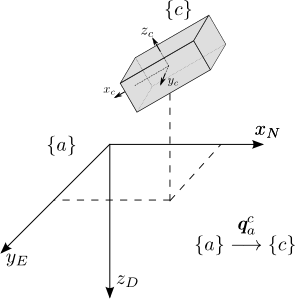
\includegraphics[scale=0.65]{images/Schema_situation.png}
\caption{Definition of the scene with 2 frame:  a fixed frame NED (North East Down) noted $\{a\}$ and a moving frame object noted $\{c\}$}
\label{Schema_situation}
\end{figure}

%
%\begin{lstlisting}[caption=Exemple of utilisation in C++,label=code]
%// om_exemple.cpp
%#include <om.h>
%
%using namespace om;
%
%void main(int argc, char** argv){
%
%	// 
%	SensorFusionManager manager;
%
%	//if calibration is necessary
%	manager.calibration();
%	
%	// while IMU send data
%	while( isData ){
%
%		// set all IMU data at time t
%		manager.setGyroscopeData(gyro_x,gyro_y,gyro_z);	
%		manager.setAccelerometerData(acc_x,acc_y,acc_z);
%		manager.setMagnetometerData(mag_x,mag_y,mag_z);
%		
%		// get different kind of output according to user's choices
%		
%		// quaternion
%		Quaternion q_est = manager.getAttitude<Quaternion>(); 
%		
%		//  rotation matrix
%		Matrix R = manager.getAttitude<Matrix>(); 
%		
%		//  axis angle
%		AxisAngle axisAngle = manager.getAttitude<Matrix>(); 
%		...
%	}
%}
%
%\end{lstlisting}

We are also working on the establishment of a dynamic sensor calibration process on all component of the IMU. We insist on the dynamic aspect. Indeed, firstly, it allows  the library to be adaptable to any kind of IMU, but also to improve the performance without requesting some effort from the user.
